\noindent\textbf{INTRODUÇÃO}
$\!$\\

Há anos criam-se máquinas que podem ser consideradas inteligentes, dada a complexidade de suas tarefas. Entretanto, uma atenção especial vem sendo direcionada às máquinas que possuem a capacidade de aprender, ou evoluir com as experiências, isto é, não necessariamente é preciso ensiná-las como realizar essas tarefas complexas. Arthur Samuel sumarizou essa ideia em uma frase atribuída a ele \cite{koza92bookGp}:

``Como computadores podem aprender a resolver problemas sem serem explicitamente programados? Em outras palavras, como computadores podem ser feitos de modo que façam uma tarefa sem que digamos exatamente como?''

Este campo, conhecido atualmente por \textit{aprendizagem de máquinas}, ou \textit{Machine Learning}, se baseia principalmente na ideia mencionada por Arthur Samuel. Neste paradigma, a tarefa do humano é criar uma máquina complexa o suficiente que a permita o aprendizado por experiência.

Nos últimos anos, foram criadas máquinas, ou agentes, que aprendem e por consequências alguns feitos marcantes foram atingidos. \textit{AlphaGo Zero}, uma máquina que joga xadrez, pode atingir desempenhos melhores que qualquer humano. Quando criado \textit{AlphaGo Zero} não possuía informações básicas sobre o funcionamento do jogo, mas foi capaz de melhorar seu desempenho com a experiência.

A realização dessas máquinas só foi possível graças aos avanços na capacidade de processamento dos computadores e a quantidade de dados disponíveis. Por consequência, mesmo que a taxa de aprendizagem da máquina seja baixa, é possível expor o agente a um alto número de experiências.

Os algoritmos de aprendizado de máquinas podem ser vistos como uma busca, dentro de um enorme espaço de possíveis soluções candidatas. De certa forma, essa busca é guiada pelas experiências passadas de forma a maximizar uma medida de desempenho \cite{jordan15Ml}.

Em geral, é possível dividir os algoritmos de aprendizagem de máquinas em quatro categorias \cite{marsland14Ml}:

\begin{enumerate}[label={\alph*)}]
\item \textbf{Aprendizado Supervisionado}: um conjunto de exemplos de treinamento (com a resposta correta) é fornecido ao algoritmo, com base nesses dados, as respostas são generalizadas para qualquer entrada possível. Em outras palavras, os dados são fornecidos ao algoritmo, incluindo o que se espera de resposta, cabe ao programa aprender com a experiência fornecida e deduzir corretamente a solução para outras entradas.
\item \textbf{Aprendizado Não-Supervisionado}: não é fornecida a resposta correta nos exemplos de treinamento, cabe ao algoritmo categorizar as entradas de acordo com suas semelhanças.
\item \textbf{Aprendizado por Reforço}: o algoritmo recebe a informação de que a resposta esta incorreta, mas não é dito como consertá-la. A máquina realiza buscas no espaço de possíveis soluções, até que encontre a solução correta.
\item \textbf{Sistemas de Recomendação}: geram recomendações de produtos ou serviços ao buscar a previsão das preferências de um usuário. 
\end{enumerate}

A principal diferença da aprendizagem por reforço em relação às primeiras é o papel da máquina no ambiente em que ocorre o aprendizado: geralmente, para os algoritmos de aprendizagem supervisionada ou não-supervisionada, o agente não influência o sistema, isto é, suas ações no decorrer do aprendizado (ou treinamento) não afetam a dinâmica do ambiente. 

Por exemplo, algoritmos de aprendizado supervisionado podem ser utilizados para previsões no mercado de ações, enquanto a aprendizagem não-supervisionada pode agrupar clientes de acordo com suas preferências de compras. A aprendizagem por reforço possui aplicações em diversas áreas, incluindo robótica e controle. Muitos problemas em que seja natural o uso de aprendizagem por reforço podem ser abordados também por algoritmos evolucionários que utilizam programação genética.

Foi mencionado que os algoritmos de aprendizado podem ser vistos como uma busca, em um espaço enorme de possibilidades, por máquinas capazes de resolver problemas com um determinado grau de acurácia. Já que o espaço de busca por soluções é vasto, é preciso realizar essa exploração de forma adaptativa ou inteligente \cite{koza92bookGp}.

Os algoritmos evolucionários buscam soluções melhores através de um processo iterativo inteligente em que:

\begin{enumerate}[label={\alph*)}]
\item Mede-se o desempenho de diversos indivíduos, inicializados com características aleatórias.
\item Os agentes que apresentarem um bom desempenho são selecionados e têm suas características modificadas, gerando novos indivíduos com aspectos semelhantes e, possivelmente, mais aptos à resolução do problema.
\item A nova população de indivíduos é avaliada. Os agentes que apresentarem melhor desempenho são novamente selecionados e modificados.
\item O processo se repete até um critério de término pré-estabelecido.
\end{enumerate}

É possível verificar a semelhança da escolha de soluções com a seleção natural biológica, isto é, indivíduos mais aptos sobrevivem e reproduzem. As modificações das soluções selecionadas são inspiradas nos fenômenos biológicos de mutação e cruzamento genético dos genitores. Essas alterações são conhecidas como operações genéticas. Por consequência, a mutação e o cruzamento genético (também conhecido como \textit{\textit{crossover}}) são chamados de \textit{operadores genéticos}. Seguindo a mesma lógica, o programa que utiliza a metodologia descrita acima é chamado de \textit{algoritmo genético}.

Vale ressaltar que as características dos indivíduos podem ser representadas de diversas formas. Além disso, as operações genéticas podem ser aplicadas de diversas maneiras, de acordo com a estrutura do indivíduo escolhida.

A \textit{programação genética} se refere a uma categoria de algoritmo genético introduzida principalmente por John R. Koza \cite{koza92bookGp} em que \textit{programas de computador} são evoluídos. Nesse sentido, diversos problemas podem ser reformulados como uma demanda por um programa de computador que produza uma saída desejada quando uma determinada entrada seja apresentada.

A principal distinção do método introduzido por Koza se refere ao modo de \textbf{representação} dos indivíduos. Grande parte dos trabalhos realizados até a década de 90, na área de algoritmos genéticos, utilizavam representações de tamanho fixo com uma sequência de caracteres.

\begin{figure}[!h]
\centering
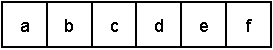
\includegraphics[width=0.35\linewidth]{01_introducao/rep_ga.pdf}
\caption{Um exemplo de indivíduo representado por uma sequência de caracteres com tamanho fixo.}
\label{fig:intro-repga}
\end{figure}

Para muitos problemas a representação natural de uma solução é um programa hierárquico de tamanho variável, ao invés de uma estrutura de comprimento fixo. Isso ocorre porque, frequentemente, não se sabe de antemão as dimensões da solução procurada.

Programas de computador hierárquicos, particularmente escritos em linguagens funcionais e/ou recursivas, podem ser facilmente representados por árvores. Por essa razão, linguagens que processam listas são escolhas naturais para abordar a programação genética \cite{koza97bookGp}.

\begin{figure}[!h]
\centering
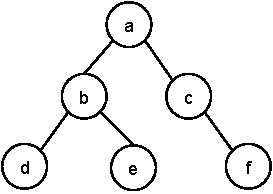
\includegraphics[width=0.4\linewidth]{01_introducao/rep_gp.pdf}
\caption{Representação de um indivíduo na \textit{programação genética}. As letras ``abcdef'' podem representar operações matemáticas, constantes ou até tomadas de decisão.}
\label{fig:intro-repgp}
\end{figure}

A estrutura da Figura \ref{fig:intro-repgp} representa um programa de computador. De fato, é possível escrever funções em LISP utilizando uma representação recursiva semelhante. Programas de computador são entidades capazes de resolver inúmeros problemas em diversos campos, por esse motivo, a programação genética pode ser utilizada em uma gama variada de situações.

Este trabalho busca aplicar a \textit{programação genética} (PG) em problemas clássicos de controle (\ref{fig:intro-gymexemplo}). O sistema do pêndulo invertido da Figura \ref{fig:intro-pendinv} é um dos problemas mais importantes na teoria de controle, principalmente pela sua natureza não-linear e instável, portanto, servirá como estudo de caso básico para este trabalho. O objetivo consiste em balancear o pêndulo utilizando a força $F$ como variável de controle, podendo esta ser aplicada na direção positiva ou negativa do eixo $x$.

\begin{figure}[!h]
\centering
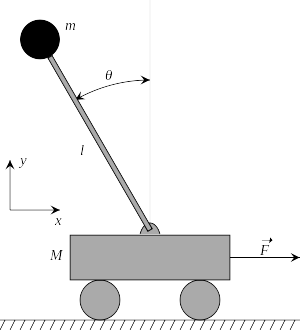
\includegraphics[width=0.4\linewidth]{01_introducao/pend_inv.png}
\captionsource{Pêndulo invertido.}{\url{https://en.wikipedia.org/wiki/Inverted_pendulum}}
\label{fig:intro-pendinv}
\end{figure}

Para realizar a avaliação dos indivíduos, é necessário uma ferramenta de simulação. Foi utilizada a biblioteca \textit{Gym} \cite{openaigym} da linguagem de programação \textit{Python}. O principal propósito desta biblioteca é criar um ambiente padronizado para testar algoritmos de aprendizagem por reforço, porém será utilizada em um problema a ser solucionado por programação genética.

\begin{figure}[H]
\centering
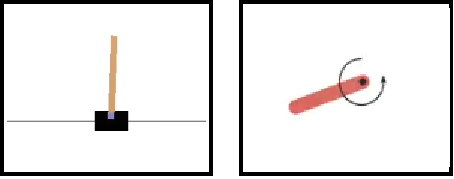
\includegraphics[width=0.5\linewidth]{01_introducao/gym_ex.pdf}
\captionsource{A biblioteca \textit{Gym} fornece alguns problemas de controle clássico como o pêndulo invertido (esquerda) e o pêndulo \textit{swingup}.}{\cite{openaigym}}
\label{fig:intro-gymexemplo}
\end{figure}

A biblioteca DEAP (\textit{Distributed Evolutionary Algorithms in Python}) é um framework de computação evolucionária designada para implementação eficiente de algoritmos evolutivos \cite{deap}. O objetivo é implementar um algoritmo de programação genética utilizando a biblioteca DEAP e evoluir a solução através do ambiente de simulação proporcionado pela biblioteca Gym.

Este trabalho busca uma abordagem didática para a implementação da \textit{programação genética} utilizando ferramentas contemporâneas. Por ser direcionado principalmente a algoritmos de \textit{aprendizagem por reforço}, existem poucas implementações de PG nos ambientes de aprendizado providos pela biblioteca Gym.

Inicialmente, é feita uma análise mais detalhada do ciclo evolutivo artificial, no contexto da programação genética. Além disso, uma verificação detalhada da representação da Figura \ref{fig:intro-repgp} e seus componentes é exigida. Então, aprofunda-se o estudo do pêndulo invertido, buscando formas de incluir na representação dos indivíduos informações importantes para a resolução do problema.

Com o modo de representação dos indivíduos definido, pode-se pensar em como inicializá-los. O conjunto de ferramentas DEAP proporciona diversos métodos que simplificam este processo. Aborda-se, então, maneiras de verificar a aptidão dos indivíduos, que representa, em suma, o desempenho de cada solução encontrada ao longo da execução do algoritmo.

Com uma medida de desempenho atribuída a cada indivíduo, pode-se implementar um método para selecionar indivíduos com base em sua aptidão. São discutidas as possíveis abordagens para essa etapa. Finalmente, as operações genéticas são implementadas em seguida.